\chapter{Methods}\label{cha:methods}

In this chapter, the selected methods for the experiments are presented and discussed.  
An understanding of the theoretical groundwork of the project from \Cref{cha:background} is assumed. Most methods are taken directly or indirectly from the source code of Gasse et al. \cite{gasse2019exact} and Gupta et al. \cite{gupta2020hybrid}, except for the choice of \gls{MLP} configurations.


\section{Dataset}\label{sec:dataset}

This section presents the selected data set and the process of generating trainable and testable data for the perceptrons. 


\subsection{Problem Instances}\label{ssec:probleminstances}

In order to evaluate the methods presented in this project to the previous advances in the field, artificially generated \gls{MILP} problems found in Gasse et al. \cite{gasse2019exact} are used to train and evaluate the models. These problems are also the standard implemented in \gls{Ecole}.
The problems are expressed as pure binary programs. The results of the algorithm are, however, generalizable to general \gls{MILP} problems, as it extends the general \gls{BnB} algorithm \cite{gasse2019exact}. 

Problems are generated in three sizes: small, medium, and large. Small instances are used for training, while medium and large problem sizes are reserved for evaluating the extended algorithm's ability to generalize on more challenging problems. These problem sizes represent what current algorithms can solve within seconds (for the small instances) and multiple minutes (for the large instances).


\subsubsection{Set covering}

Barabasi-Albert graph.
\footnote{In Gasse et al. (2019) the graph is reported to be of the type Erd\"{o}s-R\'{e}nyi, however the implementation is in fact a Barabasi-Albert graph.}

\subsubsection{Combinatorial Auction}

The combinatorial auctions problem was chosen out of the four because it has consistently proved to be the most challenging of the four problems \cite{gasse2019exact} \cite{gupta2020hybrid}. The problem is implemented by Gasse et al. \cite{gasse2019exact}, and is based on the formulation presented in Leyton-Brown et al. \cite{brown2000towards}.  

The combinatorial auctions problem is based on multi-object auctions where bidders place monetary bids on bundles (combinations) of goods, and the optimization problem is to find the bids that maximize the profit of the auctioneer \cite{brown2000towards}. The problems are considered realistic and economically oriented, and are applicable to five broad domains in which optimization is important: Proximity in Space, Paths in Space, Arbitrary Relationships, Temporal Matching, and Temporal Scheduling \cite{brown2000towards}.  


\subsubsection{Capacitated Facility Location}


\subsubsection{Maximum Independent Set}





\subsection{Expert Solution Generation}\label{ssec:expertsolutiongeneration}

The generated problems are solved using the Full Strong Branching policy, as explained in \Cref{ssec:branchingstrategy}. To not interfere with branching strategies, the application of cutting planes to the problem is restricted to the root node, i.e. before any branching decisions are made. This means that the Branch and Bound algorithm used in these experiments could be called a Cut and Branch algorithm, as is discussed in \Cref{ssec:inequalities}.
However, without loss of generality and for simplicity's sake, the algorithm will be referred to as Branch and Bound in this project despite the initial application of cutting planes.  

For every node, the \gls{SB} strategy assigns a score to every possible branching variable. The best variable to branch on according to \gls{SB} is saved explicitly and then branched on. The best candidate variable is used for training, while the \gls{SB} scores are used for evaluating the learned strategy. The placement of the selected variable compared to the candidate variables will be used to generate a top-k accuracy score, to evaluate whether the algorithm is able to select among the top variables to branch on.  


\subsection{Branching Variable Features}

At every node, i.e. for every branching decision, available features for every possible branching variable is saved. 
In total, 92 features per variable are saved, the same features as are described in the Gupta et al. \cite{gupta2020hybrid}\footnote{This is presented in Table 1 and 2 in the supplement of Gupta et al. \cite{gupta2020hybrid} article, however, there appears to be mistakes in the feature counts.}, with reference to Khalil et al. \cite{khalil2016learning}.

The variable features are divided into six subcategories, and are presented in \Cref{tab:feats}. For a description on the variables, the reader is referred to the articles listed as \textit{source}. 
%
\begin{table}[h]
	\centering
	\begin{tabular}{lrl}
		\toprule
		  Feature Description & Number of variables & Source \\ 
		  \midrule
		  Variable Features & 13 & Gasse et al. \cite{gasse2019exact} \\
		  Constraint Features & 5 & Gasse et al. \cite{gasse2019exact} \\
		  Edge Features & 1 & Gasse et al. \cite{gasse2019exact} \\
		  Optimal Variable & 1 & Gasse et al. \cite{gasse2019exact} \\
		  Static Features & 18 & Khalil et al. \cite{khalil2016learning} \\
		  Dynamic Features & 54 & Khalil et al. \cite{khalil2016learning} \\
		% \addlinespace
		\bottomrule
	\end{tabular}
	\caption{Features of each variable in the data set.}\label{tab:feats}
\end{table}
%
The underlying assumption is that these features are sufficiently correlated with the optimal variable to branch on, as is given by the Strong Branching algorithm.
% math stuff here?

\section{Models}

\subsection{Multi-Layer Perceptrons}

The selected model class for the experiments is the Multi-Layer Perceptron, as this is a well-researched, simple, and computationally uncomplex model. The Multi-Layer Perceptron is taken from the hybrid model used in Gupta et al. \cite{gupta2020hybrid}.   


\subsubsection{Network Topologies}

The \gls{MLP} proposed in Gupta et al. \cite{gupta2020hybrid} is a network of three hidden layers with $ 256 $ nodes in each layer. In the following experiments, 
three network topologies of varying sizes are chosen for comparison of accuracy and efficiency. 
For MLPs, increasing the capacity of the network correlates to increasing the number of computations \cite{goodfellow2016deep}. The networks are denoted as MLP1, MLP2, MLP3, ordered from lowest to highest complexity. The topology of MLP2 is taken from the Gupta et al. \cite{gupta2020hybrid} implementation, MLP1 is the simplest possible MLP, and MLP3 is chosen to be sufficiently larger than MLP2 within reason. It is assumed that the variation in complexity will lead to differences in both variable selection accuracy and forward pass computation time. 

MLP1, shown in \Cref{fig:topo_mlp1}, is a single-layer neural network and is equivalent to finding the optimal linear combination of input parameters. A forward pass is equivalent to a single matrix multiplication. 

MLP2, shown in \Cref{fig:topo_mlp2}, has three hidden layers of width 256. A forward pass is equivalent to four matrix multiplications with subsequent application of the activation function.

MLP3, shown in \Cref{fig:topo_mlp3}, has five hidden layers of width 1024. A forward pass is equivalent to six matrix multiplications with subsequent application of the activation function.



\begin{figure}
    \centering
        
    \def\layersep{2.0cm}
    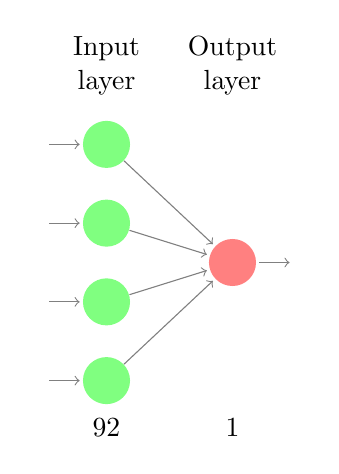
\begin{tikzpicture}[shorten >=1pt,->,draw=black!50, node distance=\layersep]
        \tikzstyle{every pin edge}=[<-,shorten <=1pt]
        \tikzstyle{neuron}=[circle,fill=black!25,minimum size=17pt,inner sep=0pt]
        \tikzstyle{input neuron}=[neuron, fill=green!50];
        \tikzstyle{output neuron}=[neuron, fill=red!50];
        \tikzstyle{hidden neuron}=[neuron, fill=blue!50];
        \tikzstyle{annot} = [text width=4em, text centered]
    
        % Draw the input layer nodes
        \foreach \name / \y in {1,...,4}
        % This is the same as writing \foreach \name / \y in {1/1,2/2,3/3,4/4}
            \node[input neuron, pin=left:] (I-\name) at (0,-\y) {};
    
       
        % Draw the output layer node
        \node[output neuron,pin={[pin edge={->}]right:}, right of=I-3, yshift=0.5cm] (O) {};
    
    
        % Connect every node in the hidden layer with the output layer
        \foreach \source in {1,...,4}
            \path (I-\source) edge (O);
    
        % Annotate the layers
        \node[annot,above of=I-1, node distance=1cm] (il) {Input layer};
        \node[annot,right of=il] {Output layer};
        
        % Annotate under
        \node[annot,below of=I-4, node distance=0.6cm](il) {92};
        \node[annot,right of=il] {1};
        
    \end{tikzpicture}
    \caption{Topology of the smaller sized MLP1 feed-forward network}
    \label{fig:topo_mlp1}
\end{figure}


\begin{figure}
    \centering
        
    \def\layersep{2.0cm}
    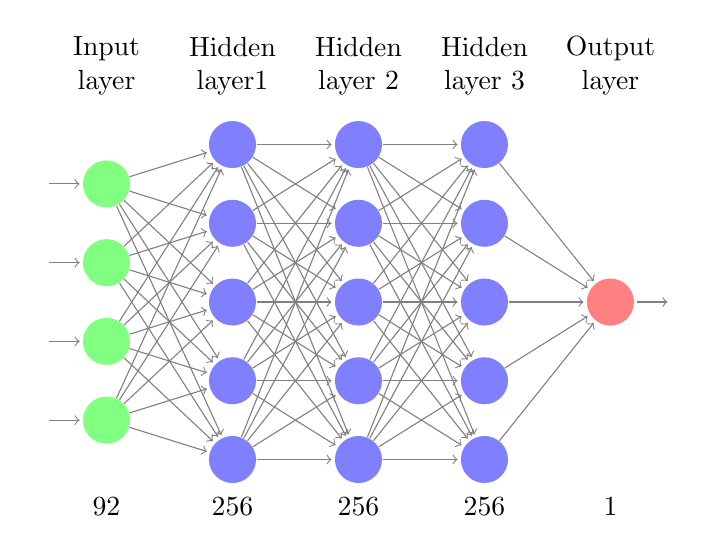
\begin{tikzpicture}[shorten >=1pt,->,draw=black!50, node distance=\layersep]
        \tikzstyle{every pin edge}=[<-,shorten <=1pt]
        \tikzstyle{neuron}=[circle,fill=black!25,minimum size=17pt,inner sep=0pt]
        \tikzstyle{input neuron}=[neuron, fill=green!50];
        \tikzstyle{output neuron}=[neuron, fill=red!50];
        \tikzstyle{hidden neuron}=[neuron, fill=blue!50];
        \tikzstyle{annot} = [text width=4em, text centered]
    
        % Draw the input layer nodes
        \foreach \name / \y in {1,...,4}
        % This is the same as writing \foreach \name / \y in {1/1,2/2,3/3,4/4}
            \node[input neuron, pin=left:] (I-\name) at (0,-\y) {};
    
        % Draw the hidden layer nodes
        \foreach \name / \y in {1,...,5}
            \path[yshift=0.5cm]
                node[hidden neuron] (H-\name) at (\layersep,-\y cm) {};
        
        \foreach \name / \y in {1,...,5}
            \path[yshift=0.5cm]
                node[hidden neuron] (H2-\name) at (\layersep*2,-\y cm) {};
                
        \foreach \name / \y in {1,...,5}
            \path[yshift=0.5cm]
                node[hidden neuron] (H3-\name) at (\layersep*3,-\y cm) {};
    
        % Draw the output layer node
        \node[output neuron,pin={[pin edge={->}]right:}, right of=H3-3] (O) {};
    
        % Connect every node in the input layer with every node in the
        % hidden layer.
        \foreach \source in {1,...,4}
            \foreach \dest in {1,...,5}
                \path (I-\source) edge (H-\dest);
        
        % Connect every node in the input layer with every node in the
        % hidden layer.
        \foreach \source in {1,...,5}
            \foreach \dest in {1,...,5}
                \path (H-\source) edge (H2-\dest);
                
        % Connect every node in the input layer with every node in the
        % hidden layer.
        \foreach \source in {1,...,5}
            \foreach \dest in {1,...,5}
                \path (H2-\source) edge (H3-\dest);
    
        % Connect every node in the hidden layer with the output layer
        \foreach \source in {1,...,5}
            \path (H3-\source) edge (O);
    
        % Annotate the layers
        \node[annot,above of=H-1, node distance=1cm] (hl) {Hidden layer1};
        \node[annot,above of=H2-1, node distance=1cm] (hl2) {Hidden layer 2};
        \node[annot,above of=H3-1, node distance=1cm] (hl3) {Hidden layer 3};
        \node[annot,left of=hl] {Input layer};
        \node[annot,right of=hl3] {Output layer};
        
        % Annotate under
        \node[annot,below of=H-1, node distance=4.6cm] (hl) {256};
        \node[annot,below of=H2-1, node distance=4.6cm] (hl2) {256};
        \node[annot,below of=H3-1, node distance=4.6cm] (hl3) {256};
        \node[annot,left of=hl] {92};
        \node[annot,right of=hl3] {1};
        
    \end{tikzpicture}
    \caption{Topology of the medium sized MLP2 feed-forward network}
    \label{fig:topo_mlp2}
\end{figure}



\begin{figure}
    \centering
        
    \def\layersep{1.6cm}
    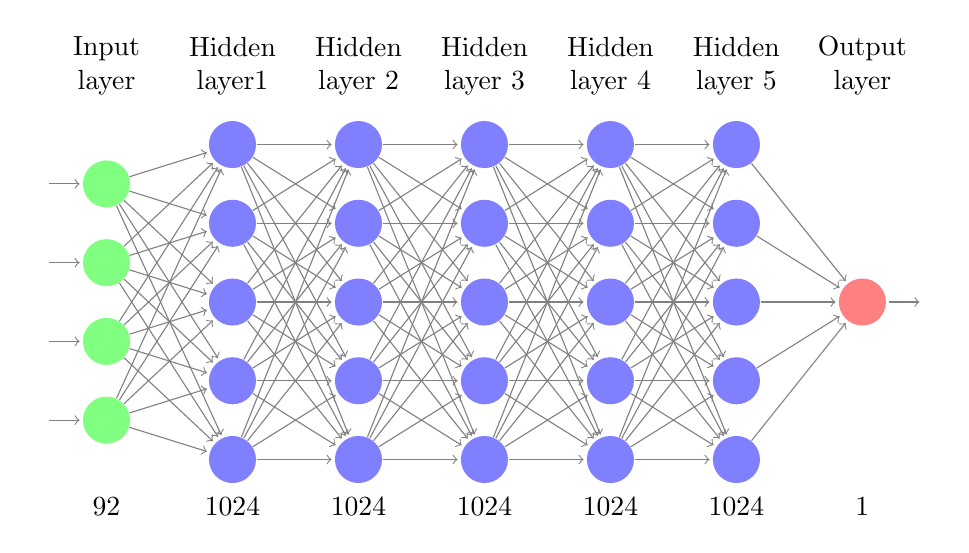
\begin{tikzpicture}[shorten >=1pt,->,draw=black!50, node distance=\layersep]
        \tikzstyle{every pin edge}=[<-,shorten <=1pt]
        \tikzstyle{neuron}=[circle,fill=black!25,minimum size=17pt,inner sep=0pt]
        \tikzstyle{input neuron}=[neuron, fill=green!50];
        \tikzstyle{output neuron}=[neuron, fill=red!50];
        \tikzstyle{hidden neuron}=[neuron, fill=blue!50];
        \tikzstyle{annot} = [text width=4em, text centered]
    
        % Draw the input layer nodes
        \foreach \name / \y in {1,...,4}
        % This is the same as writing \foreach \name / \y in {1/1,2/2,3/3,4/4}
            \node[input neuron, pin=left:] (I-\name) at (0,-\y) {};
    
        % Draw the hidden layer nodes
        \foreach \name / \y in {1,...,5}
            \path[yshift=0.5cm]
                node[hidden neuron] (H-\name) at (\layersep,-\y cm) {};
        
        \foreach \name / \y in {1,...,5}
            \path[yshift=0.5cm]
                node[hidden neuron] (H2-\name) at (\layersep*2,-\y cm) {};
                
        \foreach \name / \y in {1,...,5}
            \path[yshift=0.5cm]
                node[hidden neuron] (H3-\name) at (\layersep*3,-\y cm) {};
                
        \foreach \name / \y in {1,...,5}
            \path[yshift=0.5cm]
                node[hidden neuron] (H4-\name) at (\layersep*4,-\y cm) {};
        
        \foreach \name / \y in {1,...,5}
            \path[yshift=0.5cm]
                node[hidden neuron] (H5-\name) at (\layersep*5,-\y cm) {};
    
        % Draw the output layer node
        \node[output neuron,pin={[pin edge={->}]right:}, right of=H5-3] (O) {};
    
        % Connect every node in the input layer with every node in the
        % hidden layer.
        \foreach \source in {1,...,4}
            \foreach \dest in {1,...,5}
                \path (I-\source) edge (H-\dest);
        
        % Connect every node in the input layer with every node in the
        % hidden layer.
        \foreach \source in {1,...,5}
            \foreach \dest in {1,...,5}
                \path (H-\source) edge (H2-\dest);
                
        % Connect every node in the input layer with every node in the
        % hidden layer.
        \foreach \source in {1,...,5}
            \foreach \dest in {1,...,5}
                \path (H2-\source) edge (H3-\dest);
        
        % Connect every node in the input layer with every node in the
        % hidden layer.
        \foreach \source in {1,...,5}
            \foreach \dest in {1,...,5}
                \path (H3-\source) edge (H4-\dest);
    
        % Connect every node in the input layer with every node in the
        % hidden layer.
        \foreach \source in {1,...,5}
            \foreach \dest in {1,...,5}
                \path (H4-\source) edge (H5-\dest);
    
    
        % Connect every node in the hidden layer with the output layer
        \foreach \source in {1,...,5}
            \path (H5-\source) edge (O);
    
        % Annotate the layers
        \node[annot,above of=H-1, node distance=1cm] (hl) {Hidden layer1};
        \node[annot,above of=H2-1, node distance=1cm] (hl2) {Hidden layer 2};
        \node[annot,above of=H3-1, node distance=1cm] (hl3) {Hidden layer 3};
        \node[annot,above of=H4-1, node distance=1cm] (hl4) {Hidden layer 4};
        \node[annot,above of=H5-1, node distance=1cm] (hl5) {Hidden layer 5};
        \node[annot,left of=hl] {Input layer};
        \node[annot,right of=hl5] {Output layer};
        
        % Annotate under
        \node[annot,below of=H-1, node distance=4.6cm] (hl) {1024};
        \node[annot,below of=H2-1, node distance=4.6cm] (hl2) {1024};
        \node[annot,below of=H3-1, node distance=4.6cm] (hl3) {1024};
        \node[annot,below of=H4-1, node distance=4.6cm] (hl4) {1024};
        \node[annot,below of=H5-1, node distance=4.6cm] (hl5) {1024};
        \node[annot,left of=hl] {92};
        \node[annot,right of=hl5] {1};
        
    \end{tikzpicture}
    \caption{Topology of the larger sized MLP3 feed-forward network}
    \label{fig:topo_mlp3}
\end{figure}

\subsection{Graph Convolutional Neural Networks}

...


\subsection{Network hyperparameters}

All hyperparameters except for the amount and size of the hidden layers is consistent for all \gls{MLP}s, in order to make a fairer judgment of the accuracy/efficiency trade-off. The activation function is the \textit{Recti-Linear Unit} (ReLU), expressed as $y = \max \{ 0, x\}$. This non-linear activation function is the least computationally expensive of the common activation functions. This is consistent with Gupta et al. \cite{gupta2020hybrid}. Experiments with hyperparameters did not yield improvements, and will not be reported in this project. 


\section{Training Protocol}\label{sec:trainingprotocol}

In this section, the training protocol is presented, which explains the method to which the parameters of the \gls{MLP}s are learned.


\subsection{Loss function}

The problem is expressed as a two-class classification problem, where the classes are \textit{optimal variable} and \textit{sub-optimal variable}, respectively. The first class contains only the top variable from the strong branching evaluation. The loss function in binary classification is typically chosen as the binary cross-entropy loss function \cite{goodfellow2016deep}, calculated as:
\begin{align}
    \bm{\mathcal{L}}(\bm{\theta}) &= - \frac{1}{|\mathcal{D}|}\sum_{(\bm{x}, y) \in \mathcal{D}} \left( y_i \cdot \log( \hat y_i) + (1-y_i) \cdot \log(1 - \hat y_i) \right)\cdot w(\bm{x}_i)
\end{align}
Where $w(\bm{x}_i)$ is a depth-dependent mono-variate function in order to penalize errors for nodes close to the root more, as this has been shown to reduce solution tree size consistently, however not dramatically \cite{gupta2020hybrid}. The best weighting function was found by Gupta et al. \cite{gupta2020hybrid} to be the sigmoidal decay function, expressed as
%
\begin{align}
    w(z) &= \frac{1+e^{-0.5}}{1+e^{\; z-0.5}}
\end{align}
%
where $z$ is the depth-component of $ \bm{x} $.

It is worth noting that this depth-dependent weighting scheme will negatively impact the overall accuracy of the algorithm, in exchange for increased efficiency in solution time. This implies that comparison with methods that do not implement a similar weighting scheme, such as Khalil et al. \cite{khalil2016learning} and Gasse et al. \cite{gasse2019exact}, is not completely accurate.   


\subsection{Training method}

The parameters of the \gls{MLP} are trained via mini-batch gradient descent \cite{goodfellow2016deep}, and is performed using 
 the Adam optimizer \cite{kingma2017adam}. The adam optimizer performs gradient descent with adaptive moments in both the first and second order \cite{kingma2017adam}. 
 The batch size (number of problems processed at once) is set to 32, with 312 gradient descent steps per epoch for a maximum of 100 epochs. The learning rate is reduced upon plateaus in validation loss 
 by multiplying with $ 0.2 $. This is a well-known method to ensure convergence to a reasonably good local minimum \cite{goodfellow2016deep}.


\subsection{Computer Hardware}

Training of the \gls{MLP}s is performed on an NVIDIA RTX2070 SUPER GPU (8GB VRAM). The \gls{BnB} solution efficiency evaluations are performed with an Intel i5-2500K \gls{CPU} (4 cores, 6 threads) running at 3.31 GHz. This is less expensive hardware compared to Gasse et al. \cite{gasse2019exact} and Gupta et al. \cite{gupta2020hybrid}, particularly the CPU. Variation in processing power is assumed to have an insignificant effect on the relative solution times of the methods, however, CPUs with internal acceleration methods for matrix operations might give varying results \cite{vanhoucke2011improving}. It is assumed that the results on the chosen hardware yields a more pessimistic performance for the \gls{MLP} based methods, and will therefore not be commented on further.   


\section{Comparison Method}

The method in which the \gls{MLP}s are compared to each other and the classical branching strategies is presented in this section.


\subsection{Classical branching methods}

The accuracy and efficiency of the algorithm with the learned branching rule are evaluated against three branching strategies native to the \gls{SCIP} optimization suite. 

First is the Full Strong Branching (\gls{FSB}) strategy \cite{applegate1995finding}, the slow but accurate expert strategy that performs Strong Branching at every node for every variable. This algorithm is considered of little practical use because of the computationally heavy variable decision process \cite{achterberg2004branching}.

Pseudo-cost Branching (PB) is a fast but inaccurate branching strategy \cite{gamrath2018measuring} that chooses the variable that maximizes the lower bound improvement according to the results of previous branching decisions \cite{benchiou1971experiments}. This method does not compute anything for the candidate variables and relies only on previous results. 

Reliability Pseudo-cost Branching (\gls{RPB}) \cite{achterberg2004branching} combines \gls{FSB} and \gls{PB} by performing SB on variables with low confidence in the pseudo-costs \cite{gamrath2018measuring}. \gls{RPB} is the default branching strategy in the \gls{SCIP} \gls{BnB} solver. 


\subsection{Benchmarking}

The learned branching strategies are evaluated for both \textit{accuracy} and \textit{efficiency}. 

The accuracy of the strategies is evaluated against the expert decisions of the Full Strong Branching Algorithm. This is done by evaluating the average \textit{top-k accuracy} over an unseen test set. Top-k accuracy measures whether the chosen branching variable was within the top k choices of the Strong Branching algorithm, based on the score given to each candidate variable by the algorithm. Only the \gls{MLP}s are measured in this regard. 

The efficiency of the strategies is evaluated by exchanging the branching strategy of the optimization solver and testing on the data set with three different problem sizes, as described in \Cref{sec:dataset}. For the largest problems, solution time is limited to $ 45 $ minutes, and the number of problems the algorithm does not solve will be reported.
The execution time is compared using python's \verb|time.proc_time()| function, which returns the \gls{CPU} process time \cite{rossum2009python}. 

The number of nodes processed by the algorithm will also be reported. Fewer nodes are not necessarily indicative of a better algorithm, however, this will be an important comparison, as it gives a proxy measurement of the accuracy/efficiency trade-off for the algorithms. 


\section{Ecole}\label{sec:ecole}

\cite{prouvost2020ecole}.


\section{Development Environment}

The project is run on only Open Source Software, in order to support and further develop the commonly available tools for machine learning and mathematical programming. 

The project code is written in 
\verb|python 3.7.9|, and uses               
\verb|pytorch 1.6.0| for the machine learning models.           

For \gls{GPU} accelerated training, 
\verb|cudnn 7.6.5| and 
\verb|cudatoolkit 10.2.89| is used. 

The optimization problems are solved using the \verb|SCIP 7.0.2| Optimization Suite, using the 
\verb|SoPlex 4.0.1| linear programming solver to solve the relaxed problems. The Python interface
\verb|PySCIPOpt 3.0.4| is used to generate variable data and substitute branching strategies.
